\NeedsTeXFormat{LaTeX2e}
\documentclass	[12pt]{article}
\usepackage[pdftex]{color,graphicx}

\usepackage{graphicx,caption,subcaption}
\begin{document}

\title{\bf{Integrated Data Analysis of the DIII-D Density Profile}}
\author{L. Stagner \& W.W. Heidbrink \\ University of California--Irvine, Irvine, California, USA}
\date{}
\maketitle
\begin{abstract}
\end{abstract}
\section{Introduction}
Introstuff \cite{sivia2006data}

\section{Integrated Data Analysis}
stuff
\subsection{Bayesian basics}
stuff
\subsection{Mathematical Formulation}
stuff
\subsection{Principle of Maximum Entropy}
stuff
\subsection{Combining of multiple diagnostics}
stuff
\subsection{Model Comparision}

\section{Forward modeling of density diagnostics}
stuff
\subsection{Functional form of the density profile}
stuff
\subsection{Inteferometry}
stuff
\subsection{Reflectometry}
stuff
\subsection{Thomson scattering}
stuff
\subsection{Beam emission spectroscopy}
stuff
\section{Likelihood and prior probabilities}
stuff
\subsection{Priors}
stuff
\subsubsection{Parameter space priors}
stuff
\subsubsection{Data space priors}
stuff
\subsection{Likelihoods}
stuff
\subsubsection{Interferometry}
stuff
\subsubsection{Reflectometry}
stuff
\subsubsection{Thomson scattering}
stuff
\subsubsection{Beam emission spectroscopy}
stuff
\subsubsection{Combined likelihood probability}
stuff
\section{Total posterior probability}
stuff
\subsection{Exploring the posterior}
stuff
\section{Representation of Error}
stuff
\section{Density profile reconstructions}
stuff
\subsection{H-mode reconstruction}
stuff
\begin{figure}[ht]
	\centering
	\includegraphics[width=12cm,keepaspectratio=true]{figures/bfit146102_00505_all5}
	\vspace{-30pt}
	\caption{Reconstruction}
\label{hi}
\end{figure}
otherstuff
\subsection{L-mode reconstruction}
stuff
\section{Determining discrepant diagnostics}
stuff
\begin{figure}[h!]
	\centering
	\begin{subfigure}[b]{0.5\textwidth}
		\centering
		\includegraphics[width=\textwidth,keepaspectratio=true]{figures/bfit146102_00505_thom5}
		\vspace{-30pt}
		\caption{Thomson scattering}
		\label{fig:ts505}
	\end{subfigure}
	\hspace{-20pt}
	\begin{subfigure}[b]{0.5\textwidth}
		\centering
		\includegraphics[width=\textwidth,keepaspectratio=true]{figures/bfit146102_00505_inter5}
		\vspace{-30pt}
		\caption{Interferometer}
		\label{fig:inter505}
	\end{subfigure} \\%  ------- End of the first row ----------------------%
	\begin{subfigure}[b]{0.5\textwidth}
		\centering
		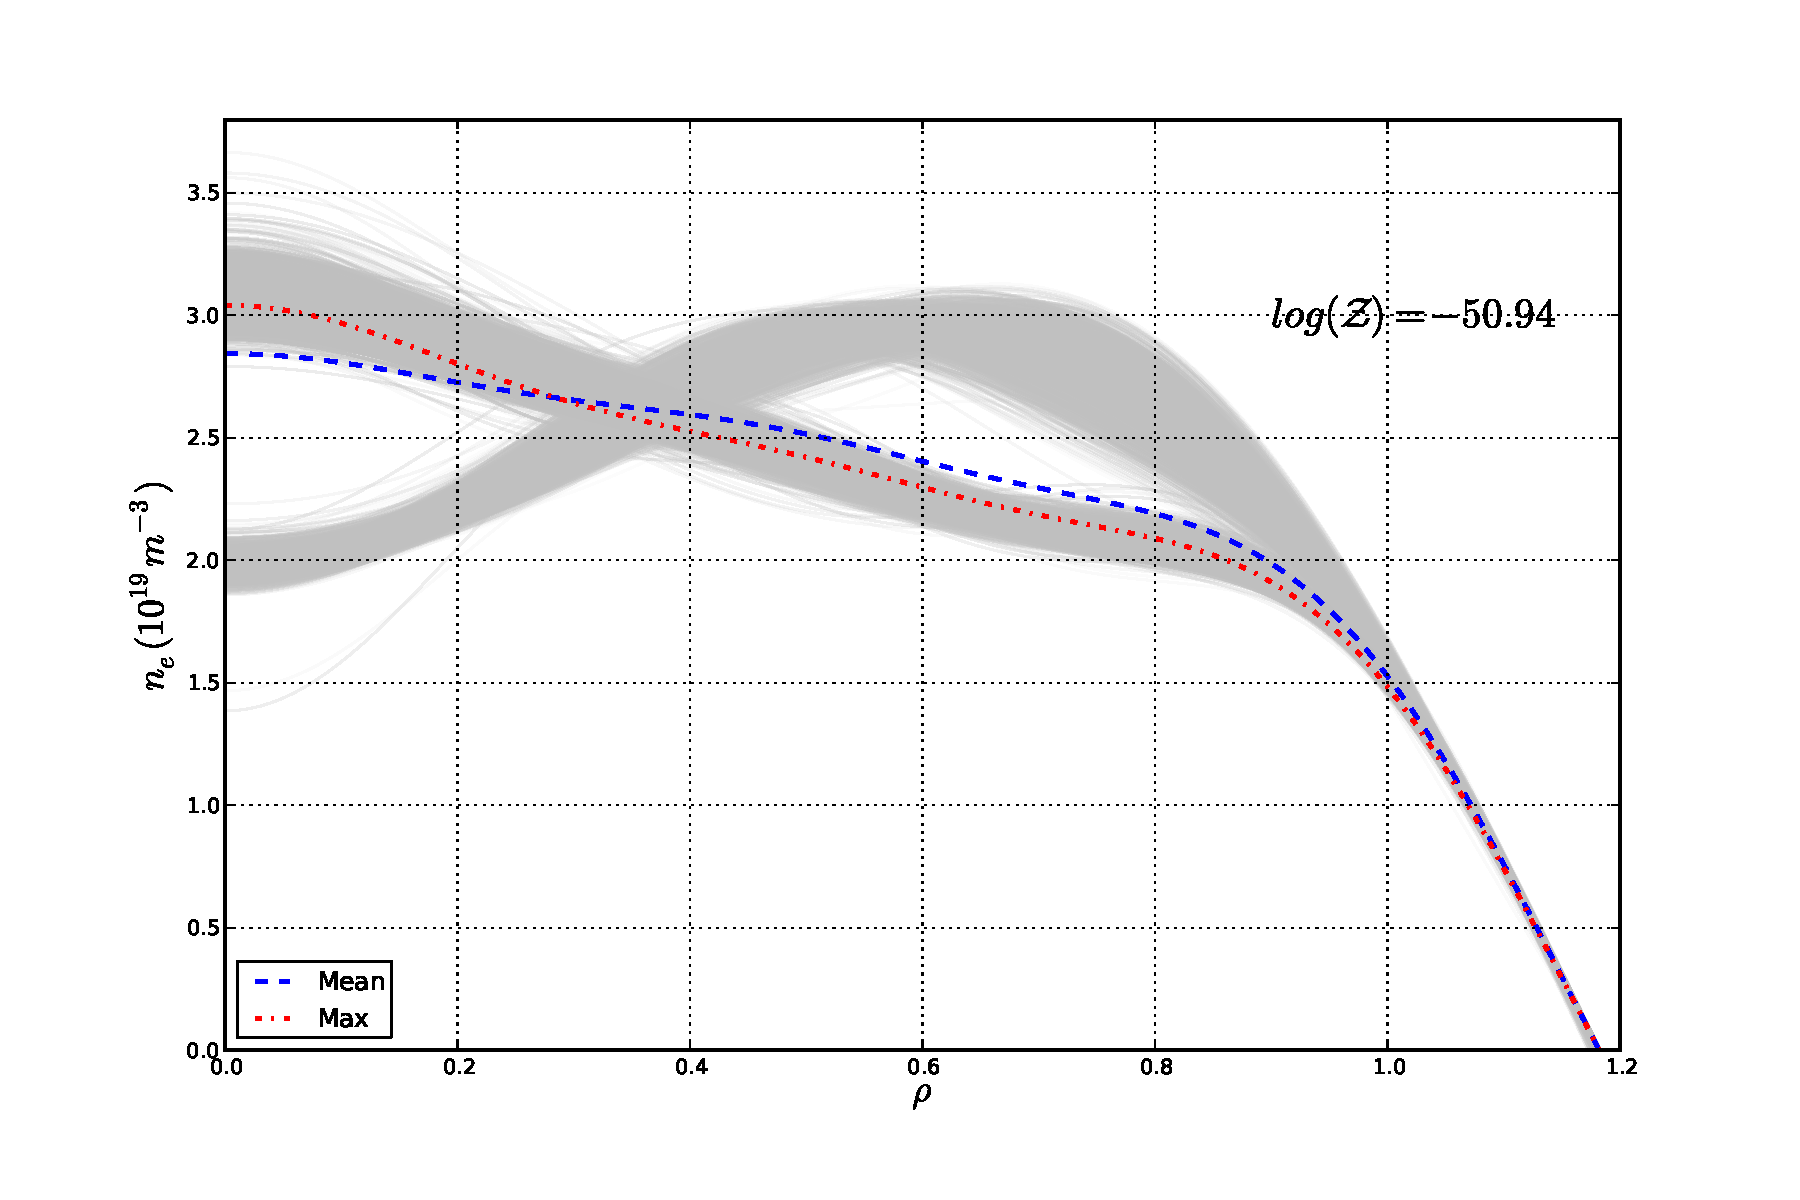
\includegraphics[width=\textwidth,keepaspectratio=true]{figures/bfit146102_00505_refl5}
		\vspace{-30pt}
		\caption{Reflectometry}
		\label{fig:refl505}
	\end{subfigure}
	\hspace{-20pt}
	\begin{subfigure}[b]{0.5\textwidth}
		\centering
		\includegraphics[width=\textwidth,keepaspectratio=true]{figures/bfit146102_00505_all5}
		\vspace{-30pt}
		\caption{Combined}
		\label{fig:all505}
	\end{subfigure}
	\caption{The l-o-n-g caption for all the subfigures (FirstFigure through FourthFigure) goes here.}
	\label{fig:dne505}
\end{figure}
\section{Conclusions and future work}
stuff

\bibliographystyle{unsrt}
\bibliography{bayes,algorithms}
\end{document}
